\section{Lineares Hashing und Wahl der Hashfunktion}

Gegeben ist die unten skizzierte leere Hashtabelle mit $q = 5$ Buckets und der Bucketgröße $b = 2$. Die Folge von Hashfunktionen sei $h_{j}(k) = k \bmod(2^{j} \cdot q), \; j = 0,1,\ldots$

\begin{minipage}{0.4\textwidth}
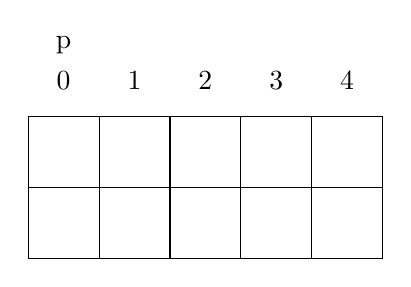
\begin{tikzpicture}
	\draw[step=.9cm] (0, 0) grid +(4.5, 1.8);

	\node at (0.45, 2.7) {p};
	\node at (0.45, 2.25) {0};
	\node at (1.35, 2.25) {1};
	\node at (2.25, 2.25) {2};
	\node at (3.15, 2.25) {3};
	\node at (4.05, 2.25) {4};
\end{tikzpicture}
\end{minipage}

\begin{enumerate}[a)]
\item Fügen Sie die folgenden Schlüssel in der angegebenen Reihenfolge in die Tabelle ein. Verwenden Sie dabei kontrolliertes Splitting mit Schwellenwert $\alpha = 0,8$. \\
49, 14, 39, 4, 119, 24, 54, 9, 74, 79, 19, 204, 59, 44, 199

\begin{solution}
\begin{minipage}{0.4\textwidth}
\begin{tikzpicture}
	%template
	\draw[step=.9cm] (0, 1.79) grid +(4.5, 1.81);
	\draw[step=.9cm] (3.5999, 0.9) grid ++(0.9, -1.8)
	  ++(-0.9, -0.9) grid ++(0.9, -1.8)
		++(-0.9, -0.9) grid ++(0.9, -1.8)
		++(-0.9, -0.9) grid ++(0.9, -1.8);
    \draw (3.6, 0) -- ++(0.9, 0)
        ++(-0.9, -0.9) -- ++(0.9, 0)
        ++(-0.9, -1.8) -- ++(0.9, 0)
        ++(-0.9, -0.9) -- ++(0.9, 0)
        ++(-0.9, -1.8) -- ++(0.9, 0)
        ++(-0.9, -0.9) -- ++(0.9, 0)
        ++(-0.9, -1.8) -- ++(0.9, 0)
        ++(-0.9, -0.9) -- ++(0.9, 0);
	\draw (4.05, 1.8) -- ++(0, -0.9)
	  ++(0, -1.8) -- ++(0, -0.9)
	  ++(0, -1.8) -- ++(0, -0.9)
	  ++(0, -1.8) -- ++(0, -0.9);
	%index
	\node at (0.45, 4.5) {p};
	\node at (0.45, 4.05) {0};
	\node at (1.35, 4.05) {1};
	\node at (2.25, 4.05) {2};
	\node at (3.15, 4.05) {3};
	\node at (4.05, 4.05) {4};
	%inserted keys
	\draw (4.05, 3.15) node{49}
	  ++(0, -0.9) node {14}
	  ++(0, -1.8) node {39}
	  ++(0, -0.9) node {4}
	  ++(0, -1.8) node {119}
	  ++(0, -0.9) node {24}
	  ++(0, -1.8) node {54}
	  ++(0, -0.9) node {9}
	  ++(0, -1.8) node {74};
	%hash functions
	\node at (2.25, -9.50) {\dashbox{1}(125,15){\footnotesize $h_0(k)$}};
\end{tikzpicture}
\end{minipage}
\begin{minipage}{0.55\textwidth}
Einfügen der Schlüssel 49, 14, 39, 4, 119, 24, 54, 9 und 74 lässt $\beta > \alpha$ werden: \\
\[\beta = \frac{N}{ (q \cdot 2^{L} + p) \cdot b} = \frac{9}{(5 \cdot 2^{0} + 0) \cdot 2} = \textcolor{red}{0,9}\]
\end{minipage}
\begin{minipage}{0.4\textwidth}
\begin{tikzpicture}
	%template
  \draw[step=.9cm] (0, 1.79) grid +(5.4, 1.81);
	\draw[step=.9cm] (3.5999, 0.9) grid ++(0.9, -1.8)
	  ++(-0.9, -0.9) grid ++(0.9, -1.8)
		++(-0.9, -0.9) grid ++(0.9, -1.8)
		++(-0.9, -0.9) grid ++(0.9, -1.8);
    \draw (3.6, 0) -- ++(0.9, 0)
        ++(-0.9, -0.9) -- ++(0.9, 0)
        ++(-0.9, -1.8) -- ++(0.9, 0)
        ++(-0.9, -0.9) -- ++(0.9, 0)
        ++(-0.9, -1.8) -- ++(0.9, 0)
        ++(-0.9, -0.9) -- ++(0.9, 0)
        ++(-0.9, -1.8) -- ++(0.9, 0)
        ++(-0.9, -0.9) -- ++(0.9, 0);
	\draw (4.05, 1.8) -- ++(0, -0.9)
	  ++(0, -1.8) -- ++(0, -0.9)
	  ++(0, -1.8) -- ++(0, -0.9)
	  ++(0, -1.8) -- ++(0, -0.9);
	%index
	\node at (1.35, 4.5) {p};
	\node at (0.45, 4.05) {0};
	\node at (1.35, 4.05) {1};
	\node at (2.25, 4.05) {2};
	\node at (3.15, 4.05) {3};
	\node at (4.05, 4.05) {4};
	\node at (4.95, 4.05) {5};
	%inserted keys
	\draw (4.05, 3.15) node{49}
	  ++(0, -0.9) node {14}
	  ++(0, -1.8) node {39}
	  ++(0, -0.9) node {4}
	  ++(0, -1.8) node {119}
	  ++(0, -0.9) node {24}
	  ++(0, -1.8) node {54}
	  ++(0, -0.9) node {9}
	  ++(0, -1.8) node {74};
	%hash functions
	\node at (2.7, -9.50) {\dashbox{1}(100,15){\footnotesize $h_0(k)$}};
	\node at (4.95, -9.50) {\dashbox{1}(25,15){\footnotesize $h_1(k)$}};
	\node at (0.45, -9.50) {\dashbox{1}(25,15){\footnotesize $h_1(k)$}};
\end{tikzpicture}
\end{minipage}
\begin{minipage}{0.55\textwidth}
Splitt von Bucket 0, es werden jetzt $h_0(k)$ und $h_1(k)$ angewendet. \\
\[\beta = \frac{N}{ (q \cdot 2^{L} + p) \cdot b} = \frac{9}{(5 \cdot 2^{0} + 1) \cdot 2} = 0,75\]
\end{minipage}

\begin{minipage}{0.4\textwidth}
\begin{tikzpicture}
	%template
	\draw[step=.9cm] (0, 1.79) grid +(5.4, 1.81);
	\draw[step=.9cm] (3.5999, 0.9) grid ++(0.9, -1.8)
	  ++(-0.9, -0.9) grid ++(0.9, -1.8)
		++(-0.9, -0.9) grid ++(0.9, -1.8)
		++(-0.9, -0.9) grid ++(0.9, -1.8);
    \draw (3.6, 0) -- ++(0.9, 0)
        ++(-0.9, -0.9) -- ++(0.9, 0)
        ++(-0.9, -1.8) -- ++(0.9, 0)
        ++(-0.9, -0.9) -- ++(0.9, 0)
        ++(-0.9, -1.8) -- ++(0.9, 0)
        ++(-0.9, -0.9) -- ++(0.9, 0)
        ++(-0.9, -1.8) -- ++(0.9, 0)
        ++(-0.9, -0.9) -- ++(0.9, 0);
	\draw (4.05, 1.8) -- ++(0, -0.9)
	  ++(0, -1.8) -- ++(0, -0.9)
	  ++(0, -1.8) -- ++(0, -0.9)
	  ++(0, -1.8) -- ++(0, -0.9);
	%index
	\node at (1.35, 4.5) {p};
	\node at (0.45, 4.05) {0};
	\node at (1.35, 4.05) {1};
	\node at (2.25, 4.05) {2};
	\node at (3.15, 4.05) {3};
	\node at (4.05, 4.05) {4};
	\node at (4.95, 4.05) {5};
	%inserted keys
	\draw (4.05, 3.15) node{49}
	  ++(0, -0.9) node {14}
	  ++(0, -1.8) node {39}
	  ++(0, -0.9) node {4}
	  ++(0, -1.8) node {119}
	  ++(0, -0.9) node {24}
	  ++(0, -1.8) node {54}
	  ++(0, -0.9) node {9}
	  ++(0, -1.8) node {74}
		++(0, -0.9) node {79};
	%hash functions
	\node at (2.7, -9.50) {\dashbox{1}(100,15){\footnotesize $h_0(k)$}};
	\node at (4.95, -9.50) {\dashbox{1}(25,15){\footnotesize $h_1(k)$}};
	\node at (0.45, -9.50) {\dashbox{1}(25,15){\footnotesize $h_1(k)$}};
\end{tikzpicture}
\end{minipage}
\begin{minipage}{0.55\textwidth}
Einfügen des Schlüssels 79 lässt $\beta > \alpha$ werden: \\
\[\beta = \frac{N}{ (q \cdot 2^{L} + p) \cdot b} = \frac{10}{(5 \cdot 2^{0} + 1) \cdot 2} = \textcolor{red}{0,83}\]
\end{minipage}

\begin{minipage}{0.4\textwidth}
\begin{tikzpicture}
	%template
	\draw[step=.9cm] (0, 1.79) grid +(6.3, 1.81);
	\draw[step=.9cm] (3.5999, 0.9) grid ++(0.9, -1.8)
	  ++(-0.9, -0.9) grid ++(0.9, -1.8)
		++(-0.9, -0.9) grid ++(0.9, -1.8)
		++(-0.9, -0.9) grid ++(0.9, -1.8);
    \draw (3.6, 0) -- ++(0.9, 0)
        ++(-0.9, -0.9) -- ++(0.9, 0)
        ++(-0.9, -1.8) -- ++(0.9, 0)
        ++(-0.9, -0.9) -- ++(0.9, 0)
        ++(-0.9, -1.8) -- ++(0.9, 0)
        ++(-0.9, -0.9) -- ++(0.9, 0)
        ++(-0.9, -1.8) -- ++(0.9, 0)
        ++(-0.9, -0.9) -- ++(0.9, 0);
	\draw (4.05, 1.8) -- ++(0, -0.9)
	  ++(0, -1.8) -- ++(0, -0.9)
	  ++(0, -1.8) -- ++(0, -0.9)
	  ++(0, -1.8) -- ++(0, -0.9);
	%index
	\node at (2.25, 4.5) {p};
	\node at (0.45, 4.05) {0};
	\node at (1.35, 4.05) {1};
	\node at (2.25, 4.05) {2};
	\node at (3.15, 4.05) {3};
	\node at (4.05, 4.05) {4};
	\node at (4.95, 4.05) {5};
	\node at (5.85, 4.05) {6};
	%inserted keys
	\draw (4.05, 3.15) node{49}
	  ++(0, -0.9) node {14}
	  ++(0, -1.8) node {39}
	  ++(0, -0.9) node {4}
	  ++(0, -1.8) node {119}
	  ++(0, -0.9) node {24}
	  ++(0, -1.8) node {54}
	  ++(0, -0.9) node {9}
	  ++(0, -1.8) node {74}
		++(0, -0.9) node {79};
	%hash functions
	\node at (0.9, -9.5) {\dashbox{1}(50,15){\footnotesize $h_1(k)$}};
	\node at (3.15, -9.5) {\dashbox{1}(75,15){\footnotesize $h_0(k)$}};
	\node at (5.4, -9.5) {\dashbox{1}(50,15){\footnotesize $h_1(k)$}};
\end{tikzpicture}
\end{minipage}
\begin{minipage}{0.4\textwidth}
Splitt von Bucket 1 \\
\[\beta = \frac{N}{ (q \cdot 2^{L} + p) \cdot b} = \frac{10}{(5 \cdot 2^{0} + 2) \cdot 2} \] \[\beta = 0,71\]
\end{minipage}

\begin{minipage}{0.4\textwidth}
\begin{tikzpicture}
	%template
	\draw[step=.9cm] (0, 1.79) grid +(6.3, 1.81);
	\draw[step=.9cm] (3.5999, 0.9) grid ++(0.9, -1.8)
	  ++(-0.9, -0.9) grid ++(0.9, -1.8)
		++(-0.9, -0.9) grid ++(0.9, -1.8)
		++(-0.9, -0.9) grid ++(0.9, -1.8)
		++(-0.9, -0.9) grid ++(0.9, -1.8);
    \draw (3.6, 0) -- ++(0.9, 0)
        ++(-0.9, -0.9) -- ++(0.9, 0)
        ++(-0.9, -1.8) -- ++(0.9, 0)
        ++(-0.9, -0.9) -- ++(0.9, 0)
        ++(-0.9, -1.8) -- ++(0.9, 0)
        ++(-0.9, -0.9) -- ++(0.9, 0)
        ++(-0.9, -1.8) -- ++(0.9, 0)
        ++(-0.9, -0.9) -- ++(0.9, 0)
        ++(-0.9, -1.8) -- ++(0.9, 0)
        ++(-0.9, -0.9) -- ++(0.9, 0);
	\draw (4.05, 1.8) -- ++(0, -0.9)
	  ++(0, -1.8) -- ++(0, -0.9)
	  ++(0, -1.8) -- ++(0, -0.9)
		++(0, -1.8) -- ++(0, -0.9)
	  ++(0, -1.8) -- ++(0, -0.9);
	%index
	\node at (2.25, 4.5) {p};
	\node at (0.45, 4.05) {0};
	\node at (1.35, 4.05) {1};
	\node at (2.25, 4.05) {2};
	\node at (3.15, 4.05) {3};
	\node at (4.05, 4.05) {4};
	\node at (4.95, 4.05) {5};
	\node at (5.85, 4.05) {6};
	%inserted keys
	\draw (4.05, 3.15) node{49}
	  ++(0, -0.9) node {14}
	  ++(0, -1.8) node {39}
	  ++(0, -0.9) node {4}
	  ++(0, -1.8) node {119}
	  ++(0, -0.9) node {24}
	  ++(0, -1.8) node {54}
	  ++(0, -0.9) node {9}
	  ++(0, -1.8) node {74}
		++(0, -0.9) node {79}
	  ++(0, -1.8) node {19}
		++(0, -0.9) node {204};
	%hash functions
	\node at (0.9, -12.2) {\dashbox{1}(50,15){\footnotesize $h_1(k)$}};
	\node at (3.15, -12.2) {\dashbox{1}(75,15){\footnotesize $h_0(k)$}};
	\node at (5.4, -12.2) {\dashbox{1}(50,15){\footnotesize $h_1(k)$}};

\end{tikzpicture}
\end{minipage}
\begin{minipage}{0.4\textwidth}
Einfügen der Schlüssel 19 und 204 lässt $\beta > \alpha$ werden: \\
\[\beta = \frac{N}{ (q \cdot 2^{L} + p) \cdot b} = \frac{12}{(5 \cdot 2^{0} + 2) \cdot 2}\] \[\beta = \textcolor{red}{0,86}\]
\end{minipage}


\begin{minipage}{0.4\textwidth}
\begin{tikzpicture}
	%template
	\draw[step=.9cm] (0, 1.79) grid +(7.2, 1.81);
	\draw[step=.9cm] (3.5999, 0.9) grid ++(0.9, -1.8)
	  ++(-0.9, -0.9) grid ++(0.9, -1.8)
		++(-0.9, -0.9) grid ++(0.9, -1.8)
		++(-0.9, -0.9) grid ++(0.9, -1.8)
		++(-0.9, -0.9) grid ++(0.9, -1.8);
    \draw (3.6, 0) -- ++(0.9, 0)
        ++(-0.9, -0.9) -- ++(0.9, 0)
        ++(-0.9, -1.8) -- ++(0.9, 0)
        ++(-0.9, -0.9) -- ++(0.9, 0)
        ++(-0.9, -1.8) -- ++(0.9, 0)
        ++(-0.9, -0.9) -- ++(0.9, 0)
        ++(-0.9, -1.8) -- ++(0.9, 0)
        ++(-0.9, -0.9) -- ++(0.9, 0)
        ++(-0.9, -1.8) -- ++(0.9, 0)
        ++(-0.9, -0.9) -- ++(0.9, 0);
	\draw (4.05, 1.8) -- ++(0, -0.9)
	  ++(0, -1.8) -- ++(0, -0.9)
	  ++(0, -1.8) -- ++(0, -0.9)
		++(0, -1.8) -- ++(0, -0.9)
	  ++(0, -1.8) -- ++(0, -0.9);
	%index
	\node at (3.15, 4.5) {p};
	\node at (0.45, 4.05) {0};
	\node at (1.35, 4.05) {1};
	\node at (2.25, 4.05) {2};
	\node at (3.15, 4.05) {3};
	\node at (4.05, 4.05) {4};
	\node at (4.95, 4.05) {5};
	\node at (5.85, 4.05) {6};
	\node at (6.75, 4.05) {7};
	%inserted keys
	\draw (4.05, 3.15) node{49}
	  ++(0, -0.9) node {14}
	  ++(0, -1.8) node {39}
	  ++(0, -0.9) node {4}
	  ++(0, -1.8) node {119}
	  ++(0, -0.9) node {24}
	  ++(0, -1.8) node {54}
	  ++(0, -0.9) node {9}
	  ++(0, -1.8) node {74}
		++(0, -0.9) node {79}
	  ++(0, -1.8) node {19}
		++(0, -0.9) node {204};
	%hash functions
	\node at (1.35, -12.2) {\dashbox{1}(75,15){\footnotesize $h_1(k)$}};
	\node at (3.6, -12.2) {\dashbox{1}(50,15){\footnotesize $h_0(k)$}};
	\node at (5.85, -12.2) {\dashbox{1}(75,15){\footnotesize $h_1(k)$}};

\end{tikzpicture}
\end{minipage}
\begin{minipage}{0.4\textwidth}
Splitt von Bucket 2 \\
\[\beta = \frac{N}{ (q \cdot 2^{L} + p) \cdot b} = \frac{12}{(5 \cdot 2^{0} + 3) \cdot 2} = 0,75\]
\end{minipage}

\begin{minipage}{0.4\textwidth}
\begin{tikzpicture}
	%template
	\draw[step=.9cm] (0, 1.79) grid +(7.2, 1.81);
	\draw[step=.9cm] (3.5999, 0.9) grid ++(0.9, -1.8)
	  ++(-0.9, -0.9) grid ++(0.9, -1.8)
		++(-0.9, -0.9) grid ++(0.9, -1.8)
		++(-0.9, -0.9) grid ++(0.9, -1.8)
		++(-0.9, -0.9) grid ++(0.9, -1.8)
		++(-0.9, -0.9) grid ++(0.9, -1.8);
    \draw (3.6, 0) -- ++(0.9, 0)
        ++(-0.9, -0.9) -- ++(0.9, 0)
        ++(-0.9, -1.8) -- ++(0.9, 0)
        ++(-0.9, -0.9) -- ++(0.9, 0)
        ++(-0.9, -1.8) -- ++(0.9, 0)
        ++(-0.9, -0.9) -- ++(0.9, 0)
        ++(-0.9, -1.8) -- ++(0.9, 0)
        ++(-0.9, -0.9) -- ++(0.9, 0)
        ++(-0.9, -1.8) -- ++(0.9, 0)
        ++(-0.9, -0.9) -- ++(0.9, 0)
        ++(-0.9, -1.8) -- ++(0.9, 0)
        ++(-0.9, -0.9) -- ++(0.9, 0);
	\draw (4.05, 1.8) -- ++(0, -0.9)
	  ++(0, -1.8) -- ++(0, -0.9)
	  ++(0, -1.8) -- ++(0, -0.9)
		++(0, -1.8) -- ++(0, -0.9)
		++(0, -1.8) -- ++(0, -0.9)
	  ++(0, -1.8) -- ++(0, -0.9);
	%index
	\node at (3.15, 4.5) {p};
	\node at (0.45, 4.05) {0};
	\node at (1.35, 4.05) {1};
	\node at (2.25, 4.05) {2};
	\node at (3.15, 4.05) {3};
	\node at (4.05, 4.05) {4};
	\node at (4.95, 4.05) {5};
	\node at (5.85, 4.05) {6};
	\node at (6.75, 4.05) {7};
	%inserted keys
	\draw (4.05, 3.15) node{49}
	  ++(0, -0.9) node {14}
	  ++(0, -1.8) node {39}
	  ++(0, -0.9) node {4}
	  ++(0, -1.8) node {119}
	  ++(0, -0.9) node {24}
	  ++(0, -1.8) node {54}
	  ++(0, -0.9) node {9}
	  ++(0, -1.8) node {74}
		++(0, -0.9) node {79}
	  ++(0, -1.8) node {19}
		++(0, -0.9) node {204}
	  ++(0, -1.8) node {59};
	%hash functions
	\node at (1.35, -14.9) {\dashbox{1}(75,15){\footnotesize $h_1(k)$}};
	\node at (3.6, -14.9) {\dashbox{1}(50,15){\footnotesize $h_0(k)$}};
	\node at (5.85, -14.9) {\dashbox{1}(75,15){\footnotesize $h_1(k)$}};

\end{tikzpicture}
\end{minipage}
\begin{minipage}{0.4\textwidth}
Einfügen des Schlüssels 59 lässt $\beta > \alpha$ werden: \\
\[\beta = \frac{N}{ (q \cdot 2^{L} + p) \cdot b} = \frac{13}{(5 \cdot 2^{0} + 3) \cdot 2} = \textcolor{red}{0,81}\]
\end{minipage}

\begin{minipage}{0.4\textwidth}
\begin{tikzpicture}
	%template
	\draw[step=.9cm] (0, 1.79) grid +(8.1, 1.81);
	\draw[step=.9cm] (3.5999, 0.9) grid ++(0.9, -1.8)
	  ++(-0.9, -0.9) grid ++(0.9, -1.8)
		++(-0.9, -0.9) grid ++(0.9, -1.8)
		++(-0.9, -0.9) grid ++(0.9, -1.8)
		++(-0.9, -0.9) grid ++(0.9, -1.8)
		++(-0.9, -0.9) grid ++(0.9, -1.8);
    \draw (3.6, 0) -- ++(0.9, 0)
        ++(-0.9, -0.9) -- ++(0.9, 0)
        ++(-0.9, -1.8) -- ++(0.9, 0)
        ++(-0.9, -0.9) -- ++(0.9, 0)
        ++(-0.9, -1.8) -- ++(0.9, 0)
        ++(-0.9, -0.9) -- ++(0.9, 0)
        ++(-0.9, -1.8) -- ++(0.9, 0)
        ++(-0.9, -0.9) -- ++(0.9, 0)
        ++(-0.9, -1.8) -- ++(0.9, 0)
        ++(-0.9, -0.9) -- ++(0.9, 0)
        ++(-0.9, -1.8) -- ++(0.9, 0)
        ++(-0.9, -0.9) -- ++(0.9, 0);
	\draw (4.05, 1.8) -- ++(0, -0.9)
	  ++(0, -1.8) -- ++(0, -0.9)
	  ++(0, -1.8) -- ++(0, -0.9)
		++(0, -1.8) -- ++(0, -0.9)
		++(0, -1.8) -- ++(0, -0.9)
	  ++(0, -1.8) -- ++(0, -0.9);
	%index
	\node at (4.05, 4.5) {p};
	\node at (0.45, 4.05) {0};
	\node at (1.35, 4.05) {1};
	\node at (2.25, 4.05) {2};
	\node at (3.15, 4.05) {3};
	\node at (4.05, 4.05) {4};
	\node at (4.95, 4.05) {5};
	\node at (5.85, 4.05) {6};
	\node at (6.75, 4.05) {7};
	\node at (7.65, 4.05) {8};
	%inserted keys
	\draw (4.05, 3.15) node{49}
	  ++(0, -0.9) node {14}
	  ++(0, -1.8) node {39}
	  ++(0, -0.9) node {4}
	  ++(0, -1.8) node {119}
	  ++(0, -0.9) node {24}
	  ++(0, -1.8) node {54}
	  ++(0, -0.9) node {9}
	  ++(0, -1.8) node {74}
		++(0, -0.9) node {79}
	  ++(0, -1.8) node {19}
		++(0, -0.9) node {204}
	  ++(0, -1.8) node {59};
	%hash functions
	\node at (1.8, -14.9) {\dashbox{1}(100,15){\footnotesize $h_1(k)$}};
	\node at (4.05, -14.9) {\dashbox{1}(25,15){\footnotesize $h_0(k)$}};
	\node at (6.3, -14.9) {\dashbox{1}(100,15){\footnotesize $h_1(k)$}};
\end{tikzpicture}
\end{minipage}
\begin{minipage}{0.4\textwidth}
Splitt von Bucket 3 \\
\[\beta = \frac{N}{ (q \cdot 2^{L} + p) \cdot b} = \frac{13}{(5 \cdot 2^{0} + 4) \cdot 2}  = 0,72\]
\end{minipage}

\begin{minipage}{0.4\textwidth}
\begin{tikzpicture}
	%template
	\draw[step=.9cm] (0, 1.79) grid +(8.1, 1.81);
	\draw[step=.9cm] (3.5999, 0.9) grid ++(0.9, -1.8)
	  ++(-0.9, -0.9) grid ++(0.9, -1.8)
		++(-0.9, -0.9) grid ++(0.9, -1.8)
		++(-0.9, -0.9) grid ++(0.9, -1.8)
		++(-0.9, -0.9) grid ++(0.9, -1.8)
		++(-0.9, -0.9) grid ++(0.9, -1.8)
		++(-0.9, -0.9) grid ++(0.9, -1.1);
    \draw (3.6, 0) -- ++(0.9, 0)
        ++(-0.9, -0.9) -- ++(0.9, 0)
        ++(-0.9, -1.8) -- ++(0.9, 0)
        ++(-0.9, -0.9) -- ++(0.9, 0)
        ++(-0.9, -1.8) -- ++(0.9, 0)
        ++(-0.9, -0.9) -- ++(0.9, 0)
        ++(-0.9, -1.8) -- ++(0.9, 0)
        ++(-0.9, -0.9) -- ++(0.9, 0)
        ++(-0.9, -1.8) -- ++(0.9, 0)
        ++(-0.9, -0.9) -- ++(0.9, 0)
        ++(-0.9, -1.8) -- ++(0.9, 0)
        ++(-0.9, -0.9) -- ++(0.9, 0)
        ++(-0.9, -1.8) -- ++(0.9, 0);
	\draw (4.05, 1.8) -- ++(0, -0.9)
	  ++(0, -1.8) -- ++(0, -0.9)
	  ++(0, -1.8) -- ++(0, -0.9)
		++(0, -1.8) -- ++(0, -0.9)
		++(0, -1.8) -- ++(0, -0.9)
		++(0, -1.8) -- ++(0, -0.9)
	  ++(0, -1.8) -- ++(0, -0.9);
	%index
	\node at (4.05, 4.5) {p};
	\node at (0.45, 4.05) {0};
	\node at (1.35, 4.05) {1};
	\node at (2.25, 4.05) {2};
	\node at (3.15, 4.05) {3};
	\node at (4.05, 4.05) {4};
	\node at (4.95, 4.05) {5};
	\node at (5.85, 4.05) {6};
	\node at (6.75, 4.05) {7};
	\node at (7.65, 4.05) {8};
	%inserted keys
	\draw (4.05, 3.15) node{49}
	  ++(0, -0.9) node {14}
	  ++(0, -1.8) node {39}
	  ++(0, -0.9) node {4}
	  ++(0, -1.8) node {119}
	  ++(0, -0.9) node {24}
	  ++(0, -1.8) node {54}
	  ++(0, -0.9) node {9}
	  ++(0, -1.8) node {74}
		++(0, -0.9) node {79}
	  ++(0, -1.8) node {19}
		++(0, -0.9) node {204}
	  ++(0, -1.8) node {59}
		++(0, -0.9) node {44}
	  ++(0, -1.8) node {199};
	%hash functions
	\node at (1.8, -16.8) {\dashbox{1}(100,15){\footnotesize $h_1(k)$}};
	\node at (4.05, -16.8) {\dashbox{1}(25,15){\footnotesize $h_0(k)$}};
	\node at (6.3, -16.8) {\dashbox{1}(100,15){\footnotesize $h_1(k)$}};
\end{tikzpicture}
\end{minipage}
\begin{minipage}{0.4\textwidth}
Einfügen der Schlüssel 44 und 199 lässt $\beta > \alpha$ werden: \\
\[\beta = \frac{N}{ (q \cdot 2^{L} + p) \cdot b} = \frac{15}{(5 \cdot 2^{0} + 4) \cdot 2}  = \textcolor{red}{0,83}\]
\end{minipage}

Splitt von Bucket 4:

\begin{tikzpicture}
	%template
	\draw[step=.9cm] (0, 1.79) grid +(9, 1.81);
	\draw[step=.9cm] (3.5999, 0.9) grid ++(0.9, -1.8)
	  ++(-0.9, -0.9) grid ++(0.9, -1.8)
		++(-0.9, -0.9) grid ++(0.9, -1.8);
	\draw[step=.9cm] (8.0999, 0.9) grid ++(0.9, -1.8)
	  ++(-0.9, -0.9) grid ++(0.9, -1.8)
		++(-0.9, -0.9) grid ++(0.9, -1.8);
	\draw (4.05, 1.8) -- ++(0, -0.9)
	  ++(0, -1.8) -- ++(0, -0.9)
		++(0, -1.8) -- ++(0, -0.9);
	\draw (8.55, 1.8) -- ++(0, -0.9)
	  ++(0, -1.8) -- ++(0, -0.9)
		++(0, -1.8) -- ++(0, -0.9);

    \draw (3.6, 0) -- ++(0.9, 0)
        ++(-0.9, -0.9) -- ++(0.9, 0)
        ++(-0.9, -1.8) -- ++(0.9, 0)
        ++(-0.9, -0.9) -- ++(0.9, 0)
        ++(-0.9, -1.8) -- ++(0.9, 0)
        ++(-0.9, -0.9) -- ++(0.9, 0);
    \draw (8.1, 0) -- ++(0.9, 0)
        ++(-0.9, -0.9) -- ++(0.9, 0)
        ++(-0.9, -1.8) -- ++(0.9, 0)
        ++(-0.9, -0.9) -- ++(0.9, 0)
        ++(-0.9, -1.8) -- ++(0.9, 0)
        ++(-0.9, -0.9) -- ++(0.9, 0);
	%index
	\node at (0.45, 4.5) {p};
	\node at (0.45, 4.05) {0};
	\node at (1.35, 4.05) {1};
	\node at (2.25, 4.05) {2};
	\node at (3.15, 4.05) {3};
	\node at (4.05, 4.05) {4};
	\node at (4.95, 4.05) {5};
	\node at (5.85, 4.05) {6};
	\node at (6.75, 4.05) {7};
	\node at (7.65, 4.05) {8};
	\node at (8.55, 4.05) {9};
	%inserted keys
	\draw (4.05, 3.15) node{14}
	  ++(0, -0.9) node {4}
	  ++(0, -1.8) node {24}
	  ++(0, -0.9) node {54}
	  ++(0, -1.8) node {74}
		++(0, -0.9) node {204}
		++(0, -1.8) node {44};
	\draw (8.55, 3.15) node{\textcolor{red}{49}}
	  ++(0, -0.9) node {\textcolor{red}{39}}
	  ++(0, -1.8) node {\textcolor{red}{119}}
	  ++(0, -0.9) node {\textcolor{red}{9}}
		++(0, -1.8) node {\textcolor{red}{79}}
	  ++(0, -0.9) node {\textcolor{red}{19}}
	  ++(0, -1.8) node {\textcolor{red}{59}}
	  ++(0, -0.9) node {\textcolor{red}{199}};
	%hash functions
	\node at (4.5, -6.8) {\dashbox{1}(260,15){\footnotesize $h_1(k)$}};
\end{tikzpicture}

\[\beta = \frac{N}{ (q \cdot 2^{L} + p) \cdot b} = \frac{15}{(5 \cdot 2^{1} + 0) \cdot 2} = 0,75\]

\end{solution}

\item Welches Verhalten fällt Ihnen bei der Verteilung der Schlüssel mit Hilfe der Hashfunktion auf? Diskutieren Sie, worin dies begründet liegt und welche unterschiedlichen Strategien Sie einsetzen können, um dem entgegen zu wirken.

\begin{solution}
Durch eine ungünstige Kombination von Schlüsselwerten und gewählter Hashfunktion, findet eine sehr ungleiche Verteilung statt.
Nur ein Splitt von Bucket 4 verbessert die Verteilung der Schlüsselwerte, es kommen dennoch weiterhin übermäßig viele Overflow-Buckets zum Einsatz.
Die folgenden zwei Lösungs-Strategien können diesem Verhalten entgegen wirken:
\begin{description}
\item [Die Anzahl der Buckets anpassen:] Siehe dazu Aufgabe \ref{sec:bucketanzahl}.
\item [Die Hashfunktion optimieren:] Eine andere Möglichkeit besteht darin, eine Hashfunktion zu verwenden, die bei ungünstig verteilten Schlüsselwerten eine bessere Verteilung erzielt. Dazu gibt es verschiedene Ansätze. Beispielsweise könnte man Schlüsselwerte jeweils von hinten lesen oder kryptographische Hashfunktionen einsetzen.
Für die Wahl einer geeigneten Hashfunktion müssen Informationen über die Verteilung der Schlüsselwerte bekannt sein.
\end{description}
\end{solution}
\end{enumerate}
